\section{Recursive Generators: LFSR and LFG}

\subsection{Linear Feedback Shift Register (LFSR)}

It is incredibly fast, operates fundamentally on binary numbers (0s and 1s), and is widely used in digital electronics and simple cryptography. An LFSR consists of:

\begin{enumerate}
    \item \textbf{Shift Register:} A device that shifts its contents into adjacent positions in the register. A bit at the end of the register is shifted out, while a new bit is inserted at the opposite end.

    \item \textbf{Output Bit:} The bit at the end that is shifted out of the register.

    \item \textbf{Feedback Function:} A function that takes bits from certain positions, called \textbf{taps}, combines them using the XOR operation, and feeds the result back into the register's input position. The bits are collected before the shift.
\end{enumerate}

An $n$-bit LFSR has $2^n$ possible states. However, because the all-zero state will produce zeros indefinitely, the maximum possible period of an LFSR sequence is $2^n-1$.

\subsection{The Mathematics of LFSR}

\subsubsection{The Recurrence Relation}

The new bit $b_n$ in a Linear Feedback Shift Register (LFSR) is calculated recursively based on the previous bits. Given a register of length $k$, with feedback taps defined by coefficients $c_i$, where $c_i=1$ if the corresponding position is an active tap and $c_i=0$ otherwise, the sequence generation is governed by the following formula:
\[
b_n = \left(c_1b_{n-1}+c_2b_{n-2}+\dots+c_kb_{n-k}\right)\pmod 2.
\]

\textit{Note: In binary mathematics, addition modulo 2 is equivalent to the logical XOR operation.}

\subsubsection{Polynomial Representation and State Shifts}

This feedback relationship can be elegantly modeled using polynomials over the binary field. Let us define the characteristic polynomial $p$ and its truncated variant $\tilde{p}$ as:
\[
p(x)=x^n+c_{n-1}x^{n-1}+\dots+c_1x+c_0
\]
and
\[
\tilde{p}(x)=c_{n-1}x^{n-1}+\dots+c_1x+c_0.
\]

If the current state of the register is represented as a polynomial $q$, then:
\[
q(x)=a_{n-1}x^{n-1}+a_{n-2}x^{n-2}+\dots+a_0.
\]

A single shift of the register corresponds to multiplying the state polynomial by the indeterminate $x$:
\[
xq(x)=a_{n-1}x^n+a_{n-2}x^{n-1}+\dots+a_0x.
\]

To keep the state within the bounds of the register, we reduce this result modulo the characteristic polynomial $p$:
\[
xq(x)\pmod{p(x)}=xq(x)-a_{n-1}p(x).
\]

Expanding this modular reduction yields the polynomial configuration for the subsequent state:
\[
\begin{aligned}
xq(x)\pmod{p(x)}
={}&(a_{n-2}-a_{n-1}c_{n-1})x^{n-1}\\
&+(a_{n-3}-a_{n-1}c_{n-2})x^{n-2}
+\dots\\
&+(a_0-a_{n-1}c_1)x-a_{n-1}c_0.
\end{aligned}
\]

Since the calculations are performed over $GF(2)$, subtraction is equivalent to addition modulo 2.

This polynomial operation is adjoint to the operation of the generator. More precisely, the action of the generator on the state can be written in matrix form:
\[
X_n=AX_{n-1},
\]
where
\[
X_n=(b_n,b_{n-1},\dots,b_{n-k+1})^T.
\]

The operation on polynomials, written in matrix form, has the transposed matrix:
\[
Y_n=A^TY_{n-1}.
\]

A matrix has a maximal period if and only if its transposed matrix has a maximal period. Therefore, it is sufficient to calculate the period for the transposed matrix.

\subsubsection{Algebraic Structure and Finite Fields}

To analyze the periodicity and structural properties of the generated sequences, we look at the underlying algebraic frameworks. By the Chinese Remainder Theorem for integers, we know that if $m$ and $n$ are coprime, there exists an isomorphism:
\[
\mathbb{Z}_{mn}\rightarrow\mathbb{Z}_m\times\mathbb{Z}_n,
\]
defined by
\[
k\rightarrow(k\bmod m,\;k\bmod n).
\]

Because $m$ and $n$ are coprime, meaning that $\gcd(m,n)=1$, this representation is a one-to-one mapping and, by cardinality, a bijection. An analogous property holds for the polynomial ring over a field $K$, provided that $p_1$ and $p_2$ are coprime:
\[
K[x]/(p_1p_2)\cong K[x]/(p_1)\times K[x]/(p_2).
\]

If the characteristic polynomial $p$ of degree $n$ is irreducible over $K=\mathbb{Z}_2$, the quotient ring forms the finite field
\[
F=K[x]/(p),
\]
containing exactly $2^n$ elements. For any non-zero element $y\in F\setminus\{0\}$, Lagrange's theorem implies that its multiplicative order divides the order of the multiplicative group. Therefore:
\[
y^{2^n-1}=1.
\]

Consequently:
\[
y^{2^n-1}-1=0
\implies
\forall y\in F\setminus\{0\},\quad y^{2^n}-y=0.
\]

The equality $y^{2^n}-y=0$ also holds for $y=0$.

\subsubsection{The Role of the Least Common Multiple (LCM)}

When analyzing elements in a direct product of structures, such as
\[
y\in G_1\times G_2,
\]
the periodicity of the combined system is determined by the \textit{Least Common Multiple}, denoted by $\operatorname{lcm}$.

Mathematically, if an element $y_1$ has a period of $t_1$, meaning that
\[
y_1^{t_1}=1,
\]
and an element $y_2$ has a period of $t_2$, meaning that
\[
y_2^{t_2}=1,
\]
then the joint element
\[
y=(y_1,y_2)
\]
will return to the identity state only when both coordinates simultaneously complete full cycles. This global period is the smallest positive integer $L$ that is a multiple of both $t_1$ and $t_2$:
\[
y^{\operatorname{lcm}(t_1,t_2)}=(1,1).
\]

If $t_1$ and $t_2$ share common factors, then
\[
\operatorname{lcm}(t_1,t_2)<t_1t_2,
\]
which reduces the total period of the system. The maximum sequence length is achieved when the component periods are coprime, in which case:
\[
\operatorname{lcm}(t_1,t_2)=t_1t_2.
\]

\subsubsection{Periodicity and Minimal Polynomials}

To determine whether an LFSR sequence can achieve its maximum length, we investigate whether there exists a smaller exponent
\[
l<2^n-1
\]
such that
\[
y^l=1
\]
for all non-zero elements $y\in F$.

If
\[
\forall y\in F,\quad y^{l+1}-y=0,
\]
then the polynomial
\[
g(Y)=Y^{l+1}-Y
\]
has all $2^n$ elements of $F$ as roots. Since a non-zero polynomial of degree $l+1$ over a field can have at most $l+1$ distinct roots, it follows that:
\[
l+1\geq 2^n.
\]

Therefore:
\[
l\geq 2^n-1.
\]

Because the multiplicative group of the finite field $F$ is cyclic, there exists a primitive generator element $y\in F$ whose successive powers
\[
y^k,\qquad k=0,\dots,2^n-2,
\]
are all distinct and represent all non-zero elements of $F$.

Let $h$ be the minimal polynomial of $y$. By definition, $h(y)=0$, $h$ is monic, and its degree is minimal among all non-zero polynomials $g$ satisfying $g(y)=0$.

Consequently, $h$ must be irreducible. If there exists some polynomial $g$ such that $g(y)=0$, applying the polynomial division algorithm yields:
\[
g=qh+r,
\qquad
\deg(r)<\deg(h).
\]

Evaluating this equality at $y$ gives:
\[
g(y)=q(y)h(y)+r(y)
\implies
0=0+r(y).
\]

Since $r(y)=0$ and the degree of $r$ is strictly less than the degree of the minimal polynomial $h$, it must follow that $r=0$. Therefore, $g$ is an exact multiple of $h$:
\[
g=qh.
\]

The evaluation mapping
\[
Y\rightarrow y
\]
establishes an isomorphism from the quotient ring
\[
K[Y]/(h(Y))
\]
to the finite field $F$. Most importantly, the successive powers of the residue class of $Y$ generate every non-zero element of
\[
K[Y]/(h(Y))
\]
if and only if the generator has a maximum period.

\begin{definition}
A \textbf{primitive polynomial} is an irreducible polynomial each of whose roots generates the multiplicative group of the corresponding finite field.
\end{definition}

\textbf{Conclusion:} To achieve the maximum possible period of $2^n-1$ states without entering a shorter cycle, the characteristic polynomial $p(x)$ must be a \textbf{primitive polynomial} over $GF(2)$.

\subsection{Example: 4-Bit LFSR}

Consider a 4-bit LFSR with feedback taps at positions 3 and 4, utilizing XOR as the feedback function.

\begin{table}[h]
\centering
\begin{tabular}{c c c c c}
\toprule
\textbf{a} & \textbf{b} & \textbf{c (tap)} & \textbf{d (tap)} & \textbf{Output} \\
\midrule
\texttt{1} & \texttt{0} & \texttt{0} & \texttt{1} & \texttt{1} \\
\texttt{1} & \texttt{1} & \texttt{0} & \texttt{0} & \texttt{0} \\
\texttt{0} & \texttt{1} & \texttt{1} & \texttt{0} & \texttt{0} \\
\texttt{1} & \texttt{0} & \texttt{1} & \texttt{1} & \texttt{1} \\
\texttt{0} & \texttt{1} & \texttt{0} & \texttt{1} & \texttt{1} \\
\texttt{1} & \texttt{0} & \texttt{1} & \texttt{0} & \texttt{0} \\
\texttt{1} & \texttt{1} & \texttt{0} & \texttt{1} & \texttt{1} \\
\texttt{1} & \texttt{1} & \texttt{1} & \texttt{0} & \texttt{0} \\
\texttt{1} & \texttt{1} & \texttt{1} & \texttt{1} & \texttt{1} \\
\texttt{0} & \texttt{1} & \texttt{1} & \texttt{1} & \texttt{1} \\
\texttt{0} & \texttt{0} & \texttt{1} & \texttt{1} & \texttt{1} \\
\texttt{0} & \texttt{0} & \texttt{0} & \texttt{1} & \texttt{1} \\
\texttt{1} & \texttt{0} & \texttt{0} & \texttt{0} & \texttt{0} \\
\texttt{0} & \texttt{1} & \texttt{0} & \texttt{0} & \texttt{0} \\
\texttt{0} & \texttt{0} & \texttt{1} & \texttt{0} & \texttt{0} \\
\texttt{1} & \texttt{0} & \texttt{0} & \texttt{1} & \texttt{1} \\
\bottomrule
\end{tabular}
\caption{Example of a 4-bit LFSR with taps $c$ and $d$}
\end{table}

The final row repeats the initial state, showing that the LFSR returns to its starting configuration after visiting all $2^4-1=15$ non-zero states.


\subsection{LFSR C++ Implementation}

The implementation follows the recurrence relation directly. In every call of \texttt{next()}, the feedback bit is computed as the XOR of all selected tap bits. Then the current register is shifted by one position, the feedback bit is inserted into the most significant position, and the result is masked so that the state remains inside the selected bit width.

\cppfile[
    caption={Implementation of the LFSR transition function},
    label={lst:lfsr-next}
]{codes/lfsr/lfsr_next.cpp}

The important part of this implementation is that the output is not produced by an external random source. It is only the result of deterministic bit operations applied to the current state. Therefore, the choice of taps and the initial state decide whether the generator has a long cycle or quickly falls into a visible pattern.

\subsection{LFSR Experimental Comparison}

Three LFSR variants were compared. The first one uses a 16-bit register with a tap set that gives good behaviour in this simple experiment. The second one uses a larger 32-bit state, but only one feedback tap, which creates a very short and structured cycle. The third one changes only the tap set in the 16-bit case, showing how a small structural change can strongly affect the output.

\begin{table}[htbp]
\centering
\small
\resizebox{\textwidth}{!}{%
\begin{tabular}{|l|r|r|r|}
\hline
Parameter & Good 16-bit LFSR & Bad 32-bit single-tap LFSR & Single bad tap 16-bit LFSR \\
\hline
Seed & $0xACE1$ & $0xACE1ACE1$ & $0xACE1$ \\
Width & $16$ & $32$ & $16$ \\
Taps & $\{0,2,3,5\}$ & $\{0\}$ & $\{0\}$ \\
Output range & $[0,2^{16}-1]$ & $[0,2^{32}-1]$ & $[0,2^{16}-1]$ \\
\hline
\end{tabular}%
}
\caption{LFSR parameter sets used in the experiment}
\label{tab:lfsr-parameters}
\end{table}

For each generator, $100000$ values were used to compute basic statistics. The histogram was divided into $20$ buckets. The sequence plot and the successive-value plot were generated using $5000$ values.

\begin{table}[htbp]
\centering
\small
\resizebox{\textwidth}{!}{%
\begin{tabular}{|l|r|r|r|}
\hline
Statistic & Good 16-bit LFSR & Bad 32-bit single-tap LFSR & Single bad tap 16-bit LFSR \\
\hline
Min & $1$ & $224857447$ & $3431$ \\
Max & $65535$ & $3786203564$ & $57772$ \\
Mean & $32731.96$ & $2147483647.50$ & $32767.50$ \\
Std. dev. & $18935.33$ & $1109199008.12$ & $16924.78$ \\
One-bit ratio & $0.499462$ & $0.500000$ & $0.500000$ \\
$\chi^2$ & $2.6648$ & $103125.0000$ & $103125.0000$ \\
\hline
\end{tabular}%
}
\caption{Basic LFSR statistics computed from $100000$ outputs}
\label{tab:lfsr-statistics}
\end{table}

The good LFSR has an almost perfect one-bit ratio and a low chi-square statistic, which means that the one-dimensional histogram is close to uniform in this experiment. The bad single-tap variants also have an ideal-looking one-bit ratio, but their chi-square values are extremely large. This is the important warning: bit balance alone can look good while the sequence still visits only a small and highly structured subset of the state space.

\begin{figure}[htbp]
\centering
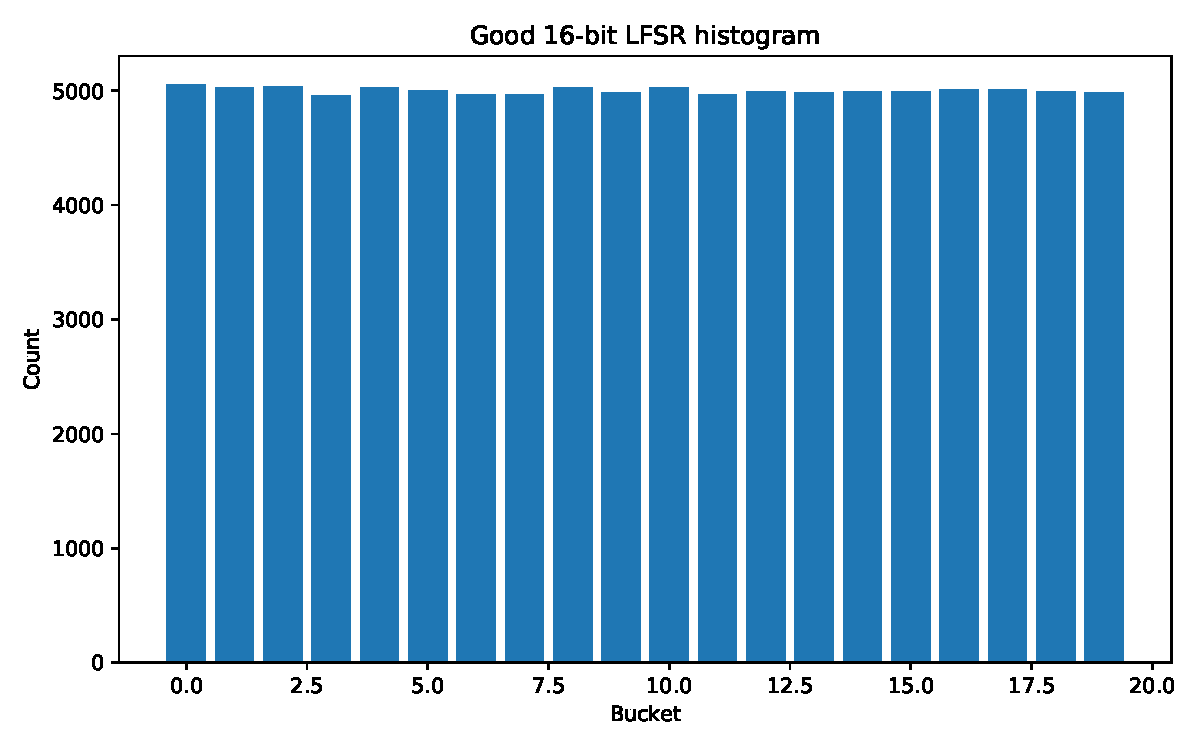
\includegraphics[width=0.48\textwidth]{figures/lfsr/good/lfsr_good_16bit_primitive_taps_histogram.pdf}
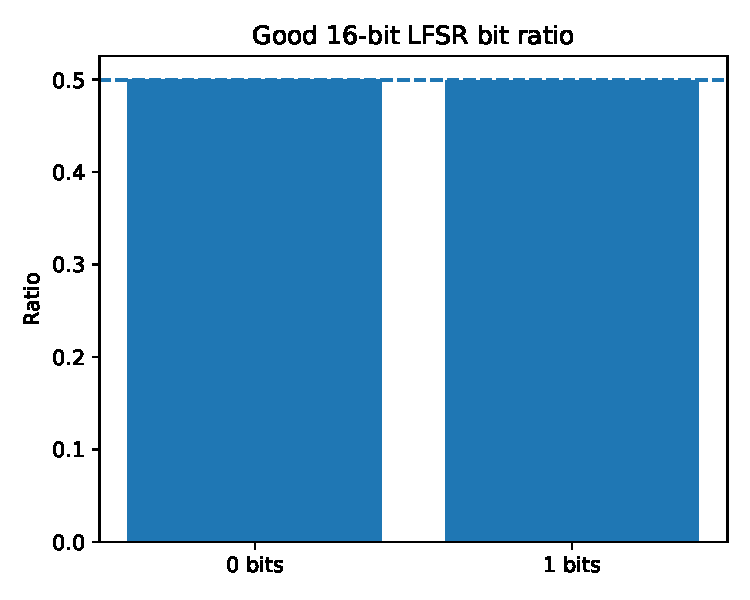
\includegraphics[width=0.48\textwidth]{figures/lfsr/good/lfsr_good_16bit_primitive_taps_bit_ratio.pdf}
\caption{Histogram and bit ratio for the good LFSR}
\label{fig:lfsr-good-hist-bits}
\end{figure}

Figure \ref{fig:lfsr-good-hist-bits} shows that the good LFSR distributes values evenly between histogram buckets. The bit ratio is close to $0.5$, so zeros and ones appear with nearly equal frequency in the output bits.

\begin{figure}[htbp]
\centering
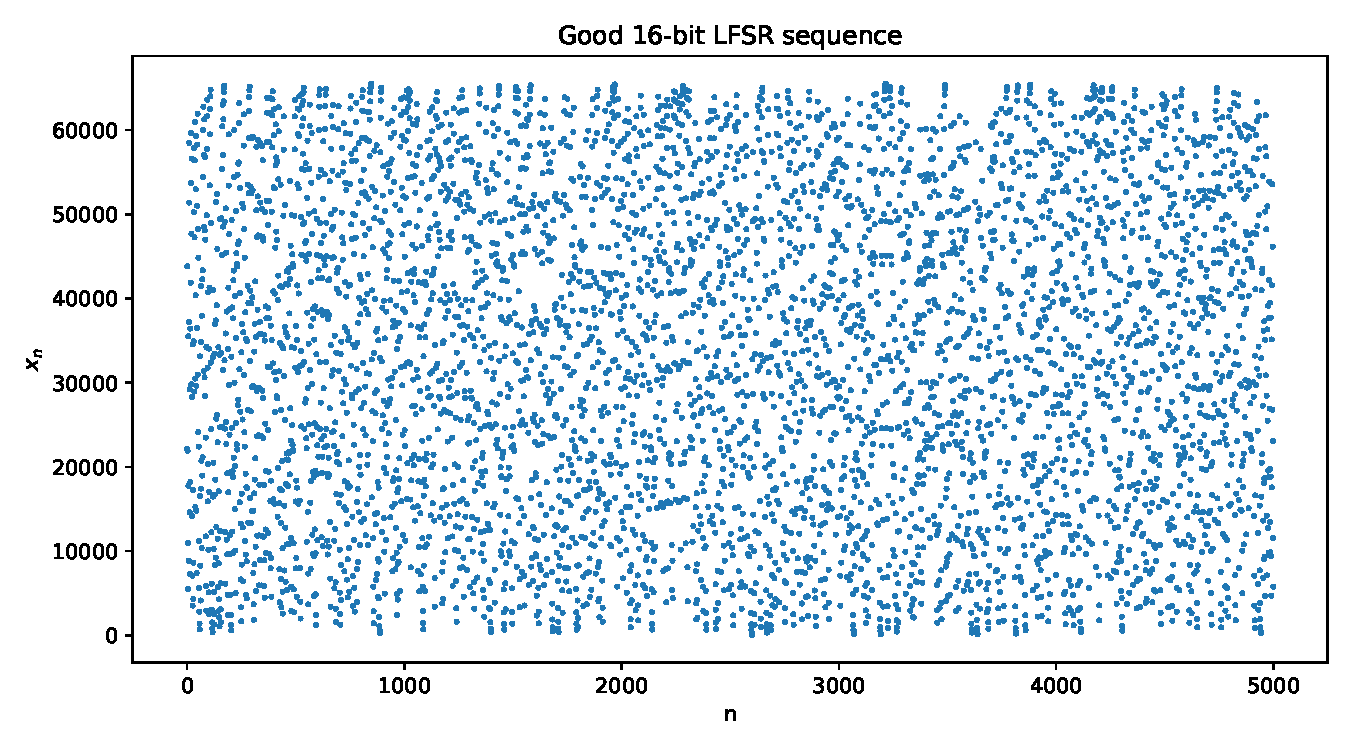
\includegraphics[width=0.48\textwidth]{figures/lfsr/good/lfsr_good_16bit_primitive_taps_sequence.pdf}
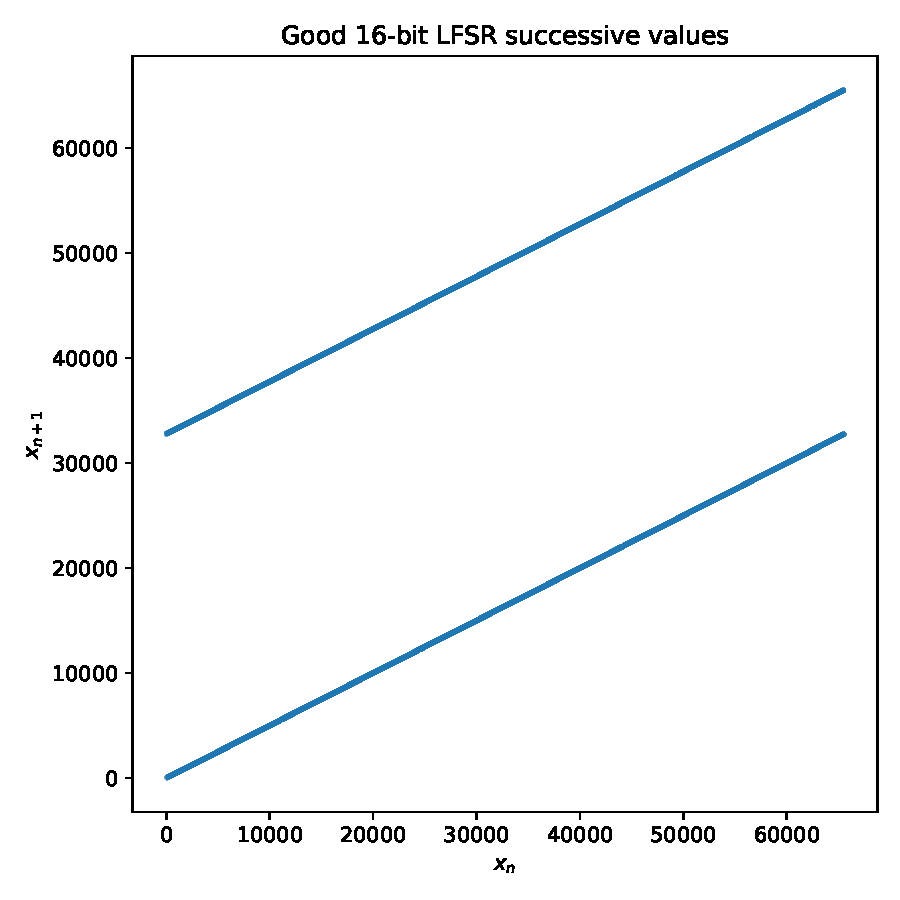
\includegraphics[width=0.48\textwidth]{figures/lfsr/good/lfsr_good_16bit_primitive_taps_successive_values.pdf}
\caption{Sequence plot and successive-value plot for the good LFSR}
\label{fig:lfsr-good-seq-succ}
\end{figure}

Figure \ref{fig:lfsr-good-seq-succ} shows that the values cover the available range without immediately collapsing into a short visible cycle. Since an LFSR is linear over $GF(2)$, this still does not make it cryptographically secure, but it is acceptable as a basic demonstration of a well-chosen feedback register.

\begin{figure}[htbp]
\centering
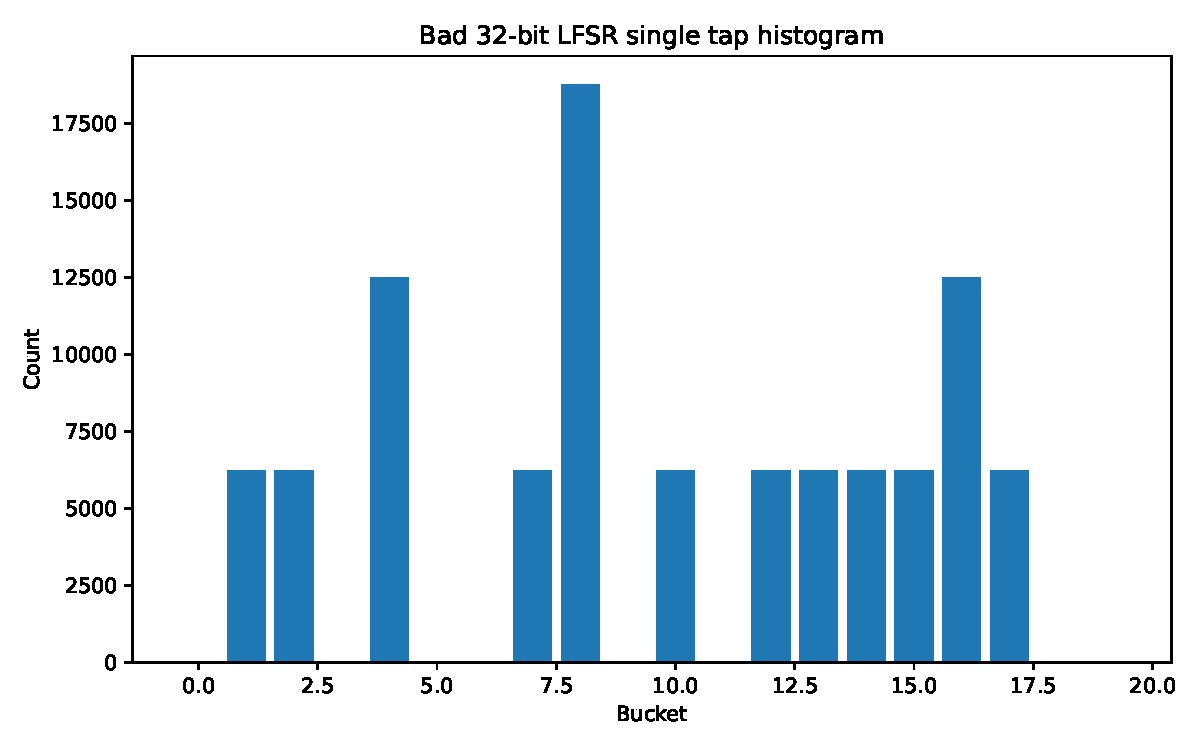
\includegraphics[width=0.48\textwidth]{figures/lfsr/bad_large_range/lfsr_bad_32bit_single_tap_histogram.pdf}
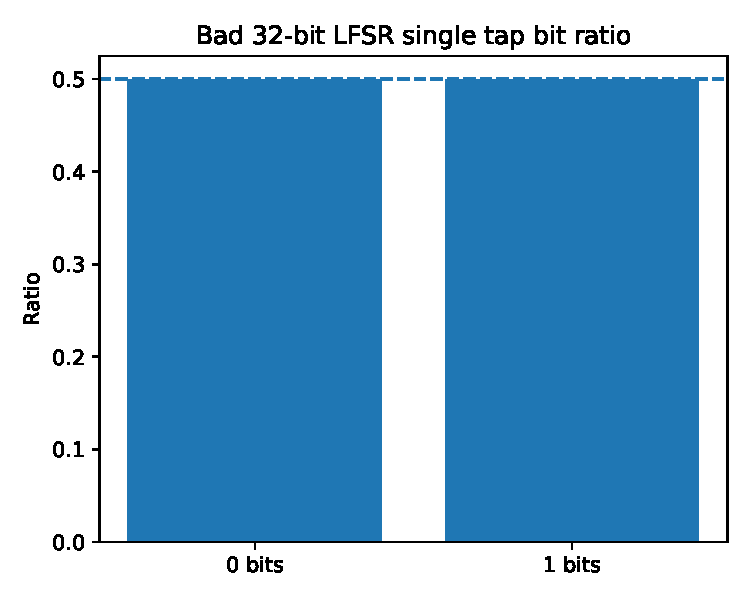
\includegraphics[width=0.48\textwidth]{figures/lfsr/bad_large_range/lfsr_bad_32bit_single_tap_bit_ratio.pdf}
\caption{Histogram and bit ratio for the bad 32-bit single-tap LFSR}
\label{fig:lfsr-bad-hist-bits}
\end{figure}

Figure \ref{fig:lfsr-bad-hist-bits} shows that using a large state is not enough. The bit ratio is exactly balanced, but the histogram is very poor. The generator has a large numerical range, but the chosen feedback rule produces a short structured cycle.

\begin{figure}[htbp]
\centering
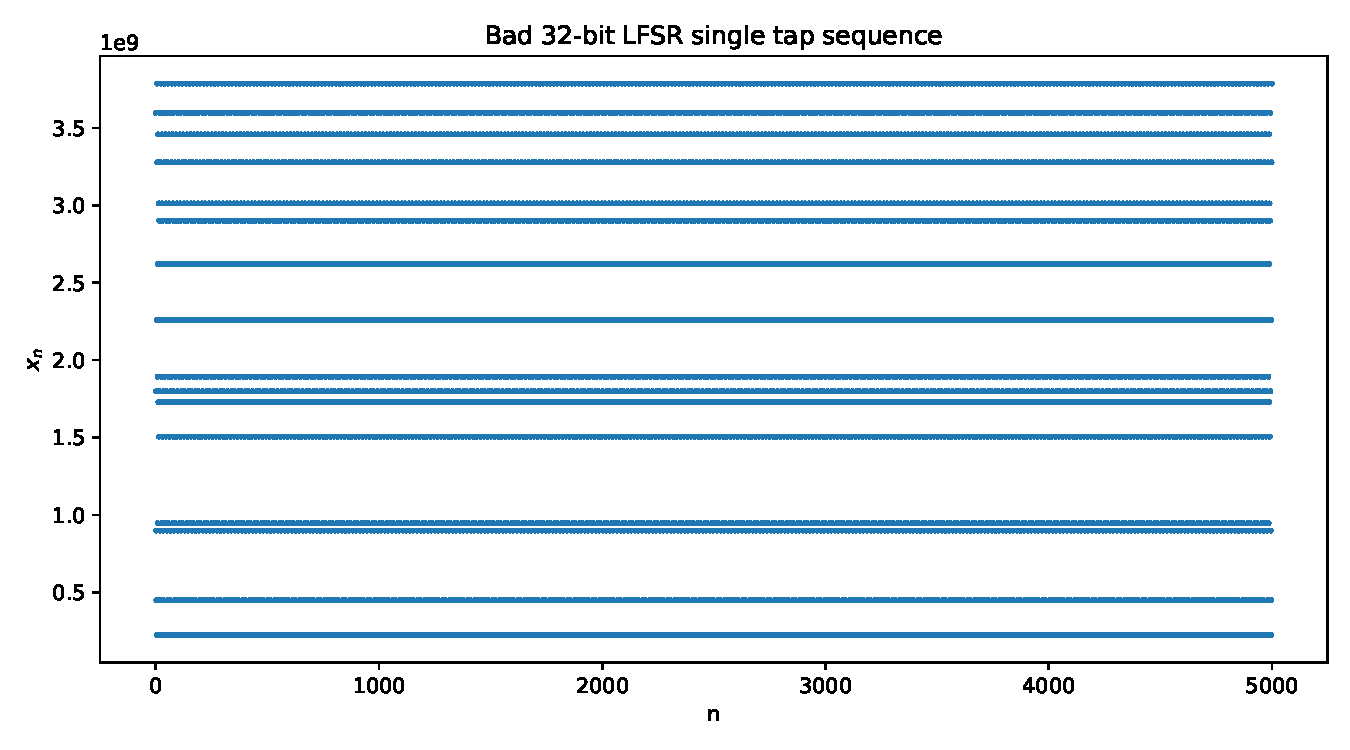
\includegraphics[width=0.48\textwidth]{figures/lfsr/bad_large_range/lfsr_bad_32bit_single_tap_sequence.pdf}
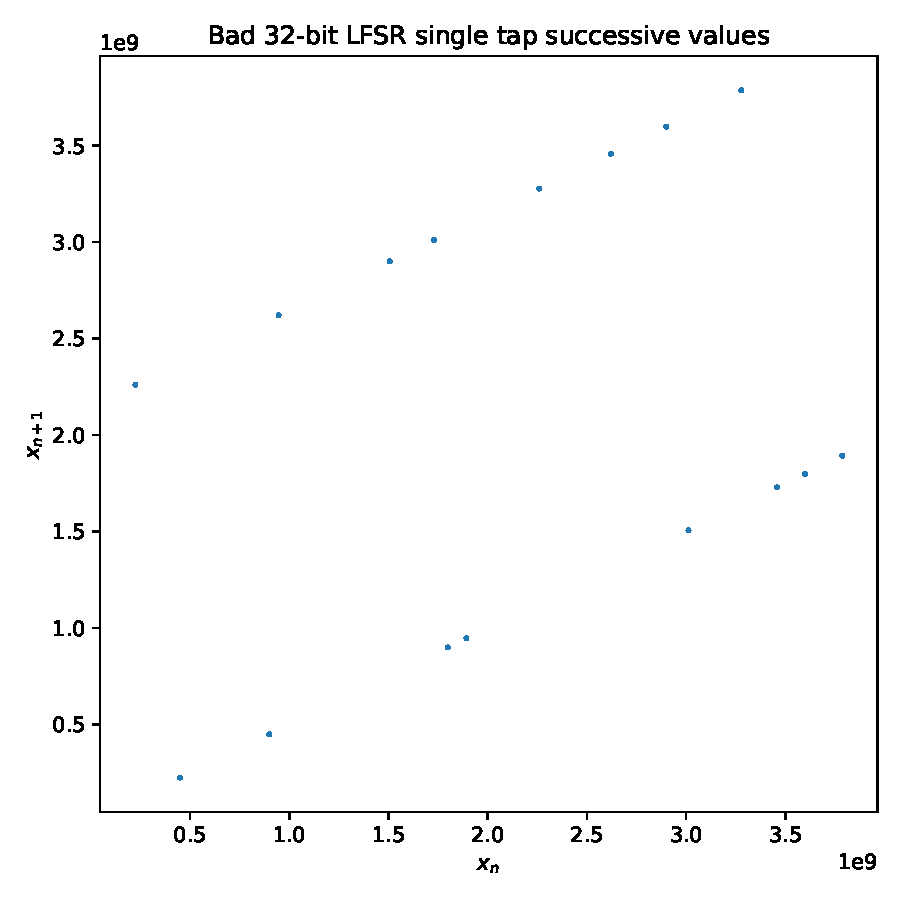
\includegraphics[width=0.48\textwidth]{figures/lfsr/bad_large_range/lfsr_bad_32bit_single_tap_successive_values.pdf}
\caption{Sequence plot and successive-value plot for the bad 32-bit single-tap LFSR}
\label{fig:lfsr-bad-seq-succ}
\end{figure}

Figure \ref{fig:lfsr-bad-seq-succ} makes the structural problem visible. The points do not fill the plane in a random-looking way. Instead, they follow a simple deterministic pattern caused by the poor tap choice.

\begin{figure}[htbp]
\centering
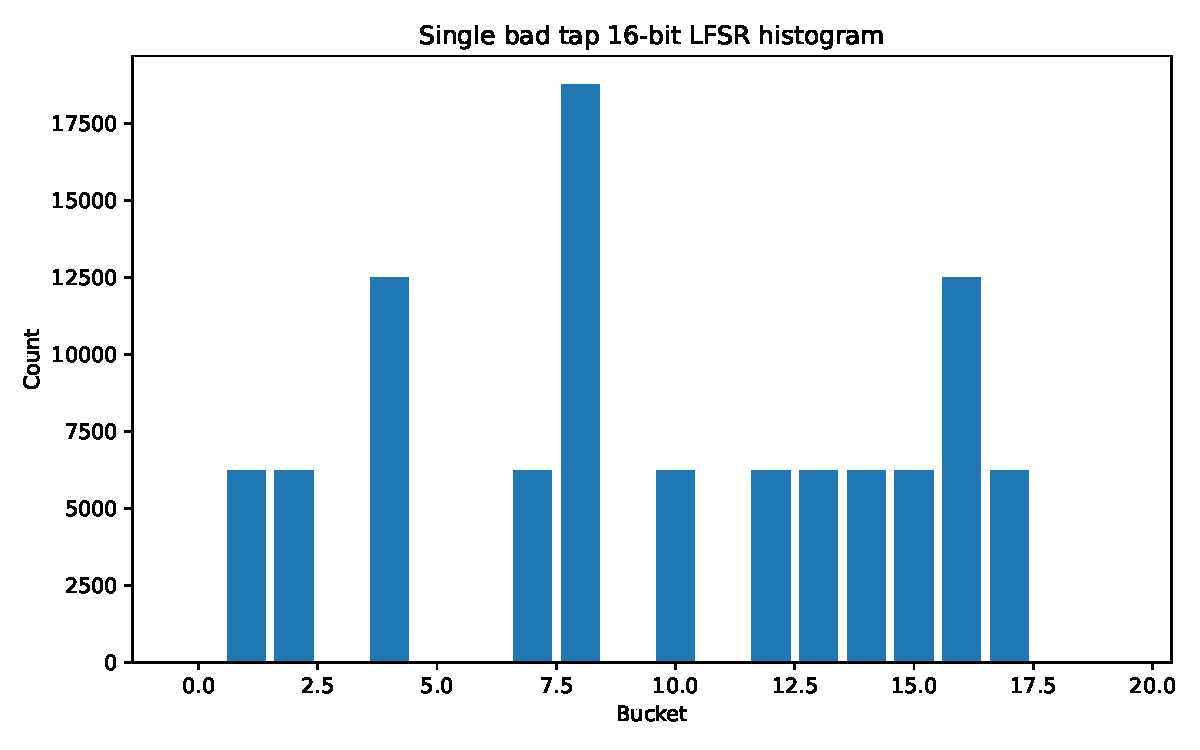
\includegraphics[width=0.48\textwidth]{figures/lfsr/single_bad_parameter/lfsr_single_bad_16bit_single_tap_histogram.pdf}
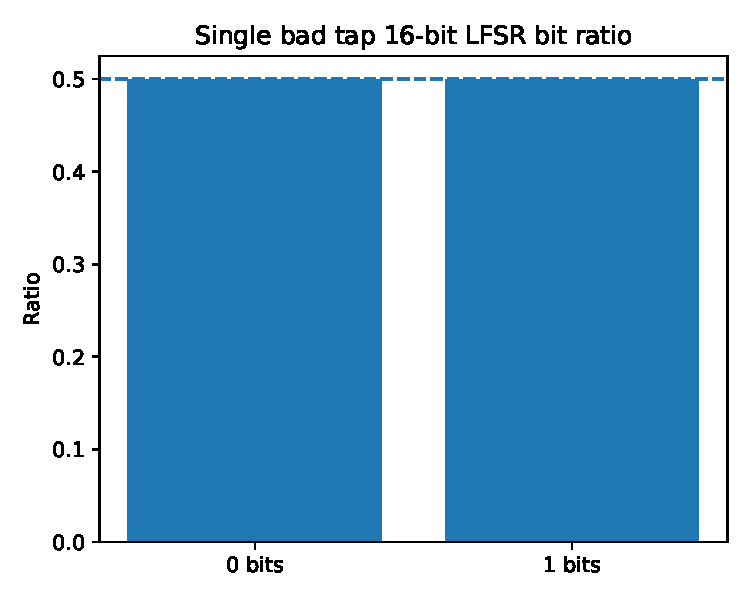
\includegraphics[width=0.48\textwidth]{figures/lfsr/single_bad_parameter/lfsr_single_bad_16bit_single_tap_bit_ratio.pdf}
\caption{Histogram and bit ratio for the 16-bit LFSR with one bad tap choice}
\label{fig:lfsr-single-bad-hist-bits}
\end{figure}

Figure \ref{fig:lfsr-single-bad-hist-bits} shows the same type of failure in a smaller register. The one-bit ratio still looks perfect, but the histogram shows that the values are not distributed correctly.

\begin{figure}[htbp]
\centering
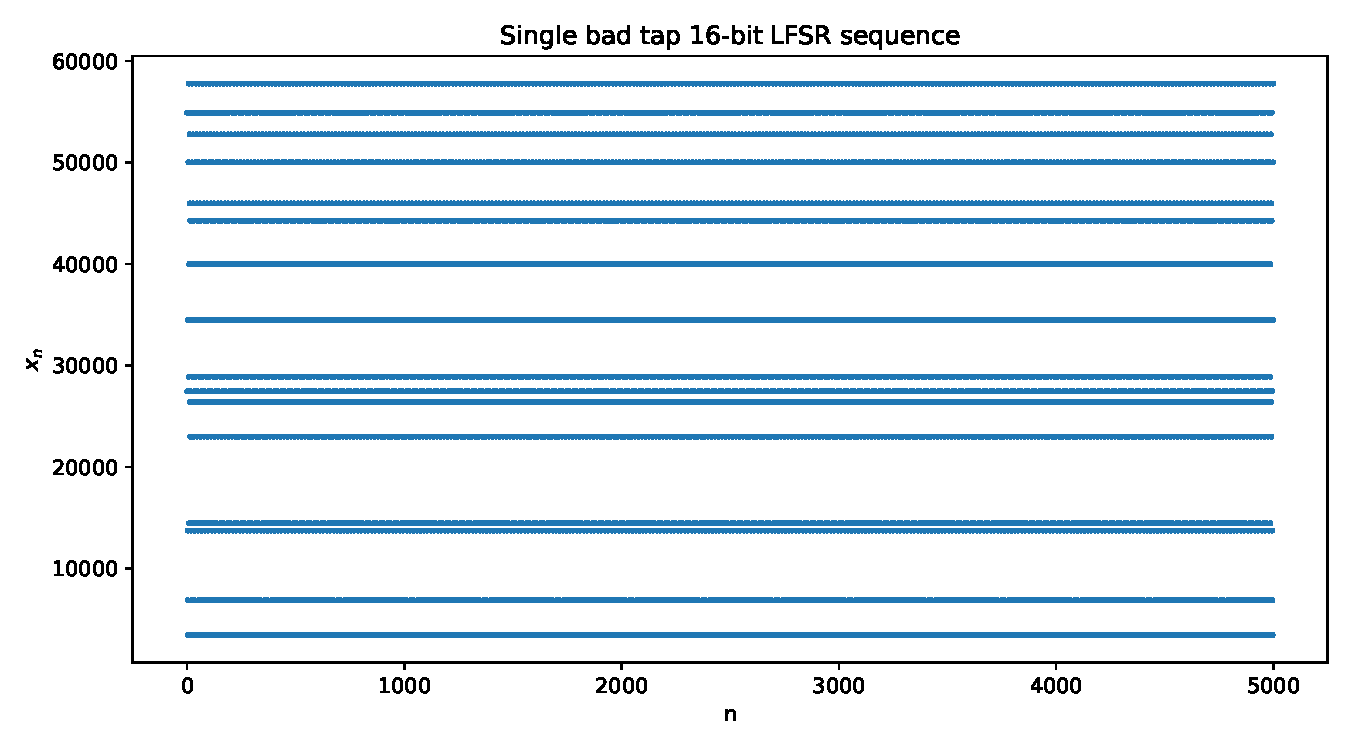
\includegraphics[width=0.48\textwidth]{figures/lfsr/single_bad_parameter/lfsr_single_bad_16bit_single_tap_sequence.pdf}
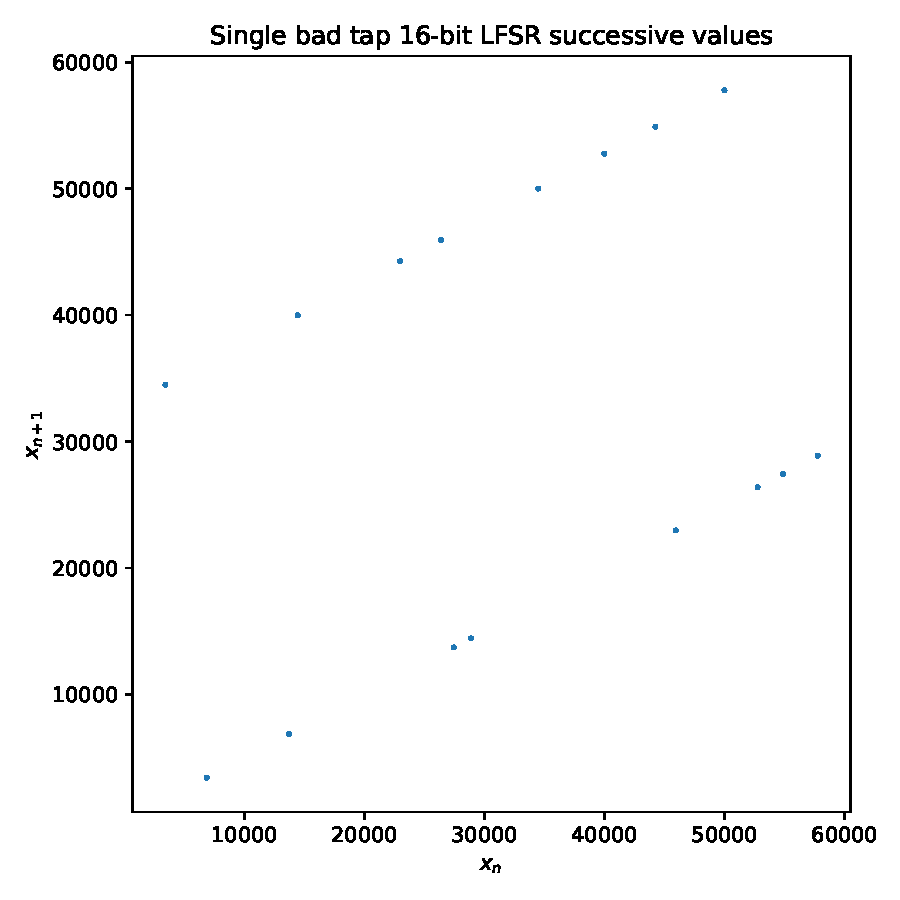
\includegraphics[width=0.48\textwidth]{figures/lfsr/single_bad_parameter/lfsr_single_bad_16bit_single_tap_successive_values.pdf}
\caption{Sequence plot and successive-value plot for the 16-bit LFSR with one bad tap choice}
\label{fig:lfsr-single-bad-seq-succ}
\end{figure}

Figure \ref{fig:lfsr-single-bad-seq-succ} confirms that changing the tap set can destroy the period and create a short deterministic structure. This is why LFSR taps should be selected using primitive polynomials rather than chosen arbitrarily.

\subsection{Lagged Fibonacci Generator (LFG)}

A Lagged Fibonacci Generator is a recursive pseudorandom number generator that generalizes the Fibonacci recurrence. Instead of using only the two immediately previous values, it combines two older values separated by fixed lags. In the additive version used here, the recurrence is
\[
x_n = (x_{n-j} + x_{n-k}) \bmod 2^{64},
\]
where $j$ and $k$ are positive integers with $j < k$. The generator stores the last $k$ values in an internal circular buffer.

The quality of an LFG depends on the choice of lags and on the initialization of the whole state array. Unlike an LCG or a simple LFSR, the seed is not just one value of the recurrence. It must be expanded into a complete initial table of values. Poor initialization may create visible patterns even when the recurrence itself has reasonable parameters.

\subsection{LFG C++ Implementation}

The implementation stores the state in an array of length equal to the long lag. The index points to the position that will be overwritten. In each call of \texttt{next()}, two previous values are selected from the circular buffer, added together, and the result replaces the oldest value.

\cppfile[
    caption={Implementation of the Lagged Fibonacci Generator transition function},
    label={lst:lfg-next}
]{codes/lfg/lagged_fibonacci_next.cpp}

The recurrence is very fast, because it only requires indexing, integer addition, and one circular-buffer update. The modulo $2^{64}$ operation is implicit for unsigned 64-bit arithmetic: overflow automatically wraps around. This makes the implementation simple, but the statistical quality still depends on good lags and a properly mixed initial state.

\subsection{LFG Experimental Comparison}

Three LFG variants were compared. The first one uses the classical additive lag pair $(24,55)$ and a mixed initial state. The second one uses very short lags $(1,2)$, which makes the recurrence much closer to the ordinary Fibonacci recurrence and increases dependence between consecutive values. The third one keeps the good lags but uses a constant initial state, showing how bad initialization can damage the generator.

\begin{table}[htbp]
\centering
\small
\resizebox{\textwidth}{!}{%
\begin{tabular}{|l|r|r|r|}
\hline
Parameter & Good LFG & Bad short-lag LFG & Constant-state LFG \\
\hline
Seed & $42$ & $42$ & constant state \\
Short lag $j$ & $24$ & $1$ & $24$ \\
Long lag $k$ & $55$ & $2$ & $55$ \\
Operation & addition mod $2^{64}$ & addition mod $2^{64}$ & addition mod $2^{64}$ \\
\hline
\end{tabular}%
}
\caption{LFG parameter sets used in the experiment}
\label{tab:lfg-parameters}
\end{table}

\begin{table}[htbp]
\centering
\small
\resizebox{\textwidth}{!}{%
\begin{tabular}{|l|r|r|r|}
\hline
Statistic & Good LFG & Bad short-lag LFG & Constant-state LFG \\
\hline
Min & $1.3171\cdot 10^{14}$ & $4.3654\cdot 10^{14}$ & $2$ \\
Max & $1.8447\cdot 10^{19}$ & $1.8447\cdot 10^{19}$ & $1.8447\cdot 10^{19}$ \\
Mean & $9.2319\cdot 10^{18}$ & $9.2302\cdot 10^{18}$ & $9.0300\cdot 10^{18}$ \\
Std. dev. & $5.3384\cdot 10^{18}$ & $5.3292\cdot 10^{18}$ & $5.4468\cdot 10^{18}$ \\
One-bit ratio & $0.499816$ & $0.505044$ & $0.494553$ \\
$\chi^2$ & $15.4312$ & $22.6568$ & $977.5000$ \\
\hline
\end{tabular}%
}
\caption{Basic LFG statistics computed from $100000$ outputs}
\label{tab:lfg-statistics}
\end{table}

The good LFG has a one-bit ratio close to $0.5$ and a moderate chi-square statistic. The short-lag generator still covers almost the whole 64-bit range, so its minimum and maximum do not immediately reveal the problem. However, its bit ratio is shifted away from $0.5$, and the recurrence has much stronger local dependence. The constant-state variant has the largest chi-square statistic, which indicates a strong distortion in the one-dimensional distribution.

\begin{figure}[htbp]
\centering
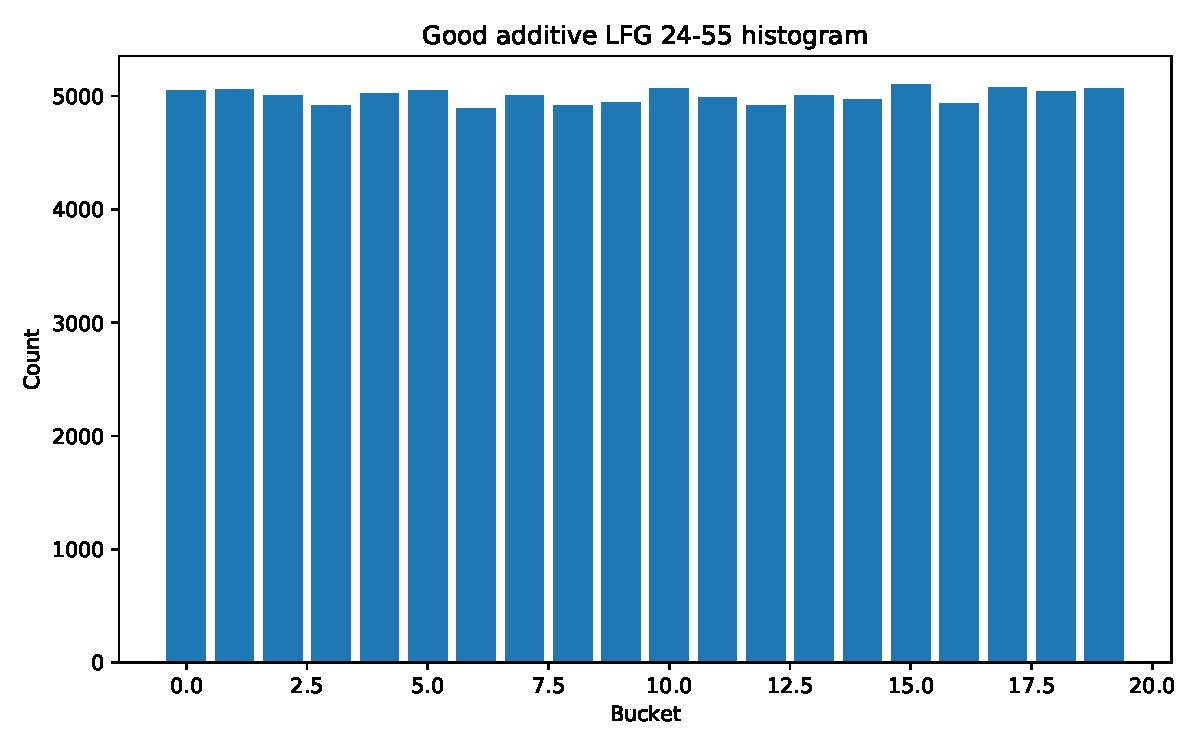
\includegraphics[width=0.48\textwidth]{figures/lfg/good/lfg_good_24_55_additive_histogram.pdf}
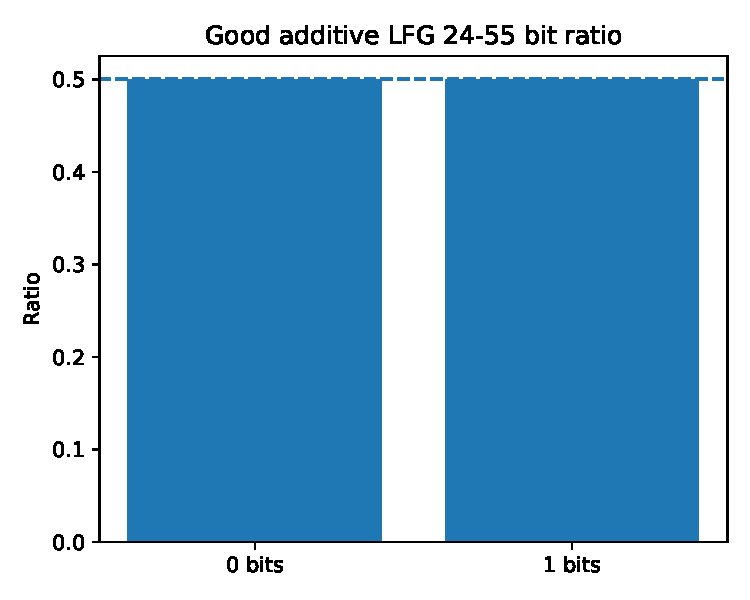
\includegraphics[width=0.48\textwidth]{figures/lfg/good/lfg_good_24_55_additive_bit_ratio.pdf}
\caption{Histogram and bit ratio for the good LFG}
\label{fig:lfg-good-hist-bits}
\end{figure}

Figure \ref{fig:lfg-good-hist-bits} shows that the good LFG produces an approximately balanced distribution in this basic test. The histogram buckets are close to each other, and the bit ratio is near the ideal value $0.5$.

\begin{figure}[htbp]
\centering
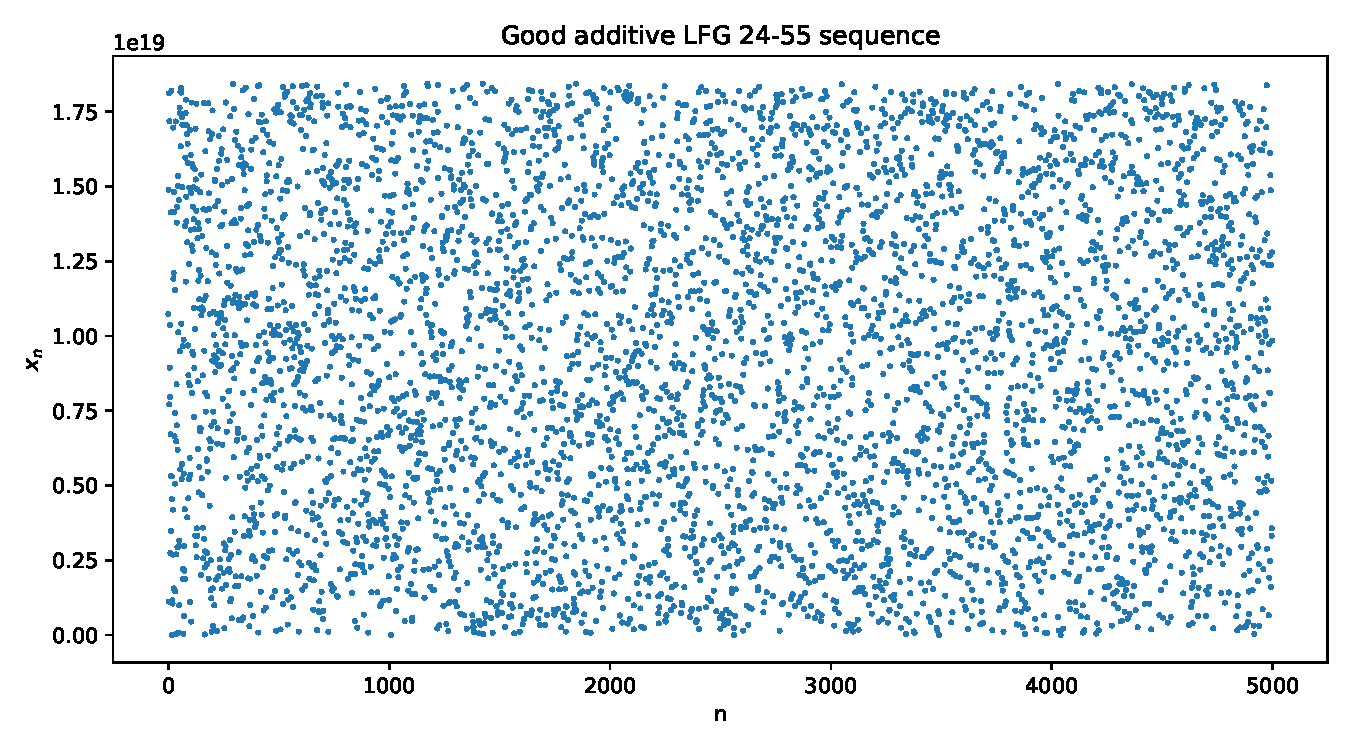
\includegraphics[width=0.48\textwidth]{figures/lfg/good/lfg_good_24_55_additive_sequence.pdf}
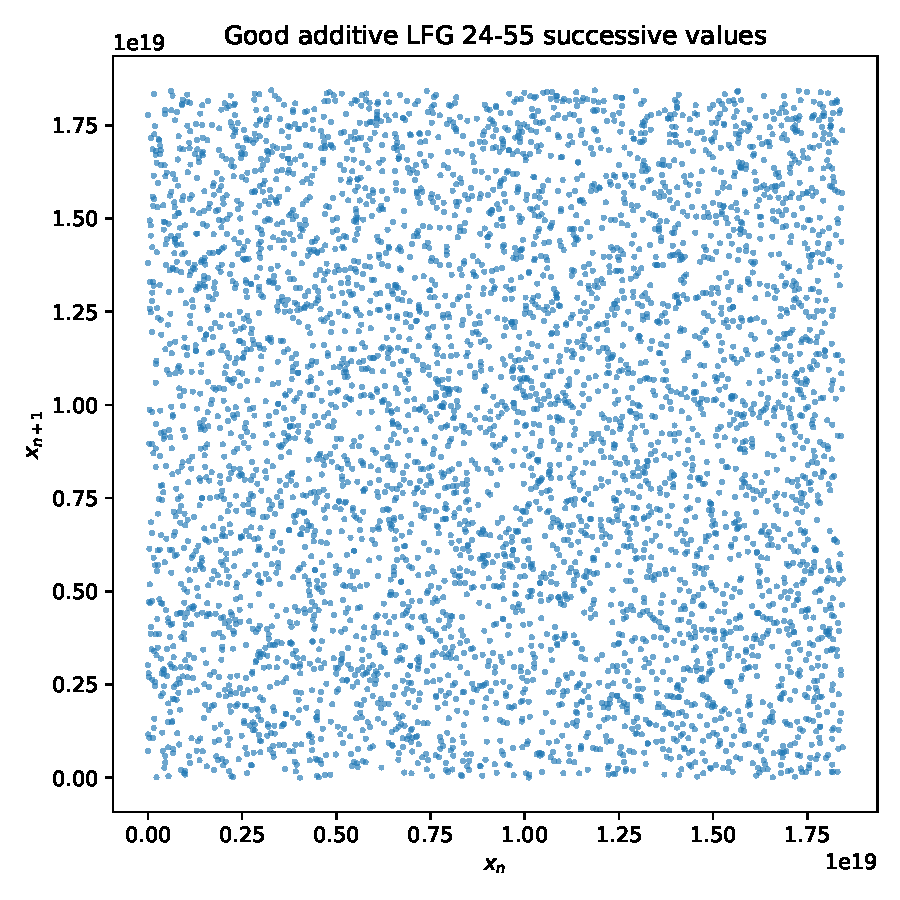
\includegraphics[width=0.48\textwidth]{figures/lfg/good/lfg_good_24_55_additive_successive_values.pdf}
\caption{Sequence plot and successive-value plot for the good LFG}
\label{fig:lfg-good-seq-succ}
\end{figure}

Figure \ref{fig:lfg-good-seq-succ} shows that the values spread across the 64-bit range. The successive-value plot does not collapse into a simple visible line, which is the expected behaviour for a reasonably initialized additive LFG.

\begin{figure}[htbp]
\centering
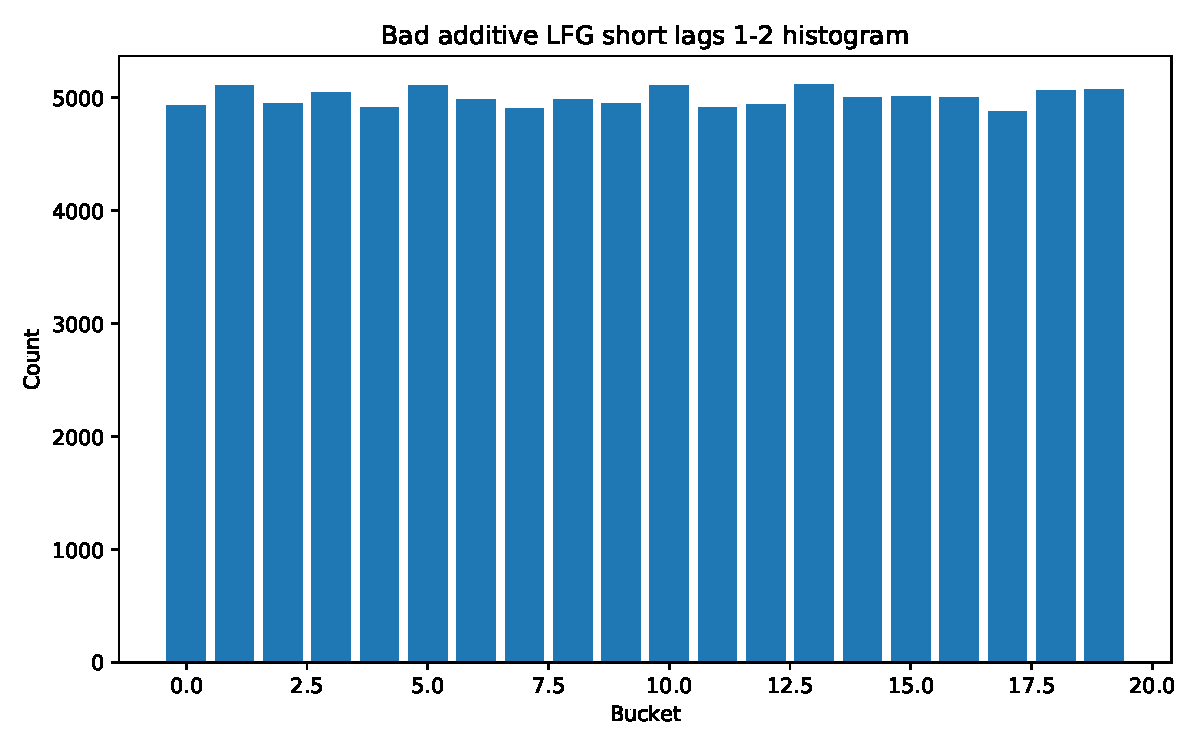
\includegraphics[width=0.48\textwidth]{figures/lfg/bad_large_range/lfg_bad_short_lags_1_2_histogram.pdf}
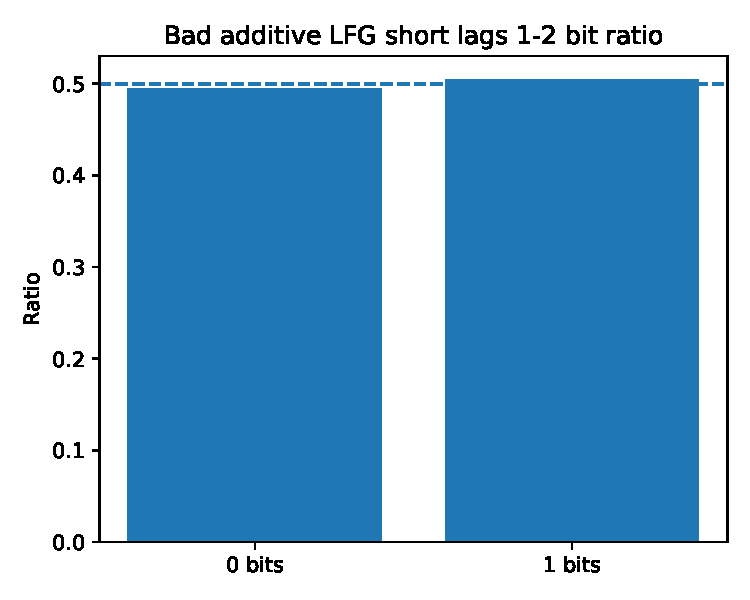
\includegraphics[width=0.48\textwidth]{figures/lfg/bad_large_range/lfg_bad_short_lags_1_2_bit_ratio.pdf}
\caption{Histogram and bit ratio for the bad short-lag LFG}
\label{fig:lfg-bad-hist-bits}
\end{figure}

Figure \ref{fig:lfg-bad-hist-bits} shows that the short-lag LFG may still look acceptable in a simple histogram, but its bit ratio is less balanced than in the good case. This illustrates that large numerical range alone does not guarantee good pseudorandom behaviour.

\begin{figure}[htbp]
\centering
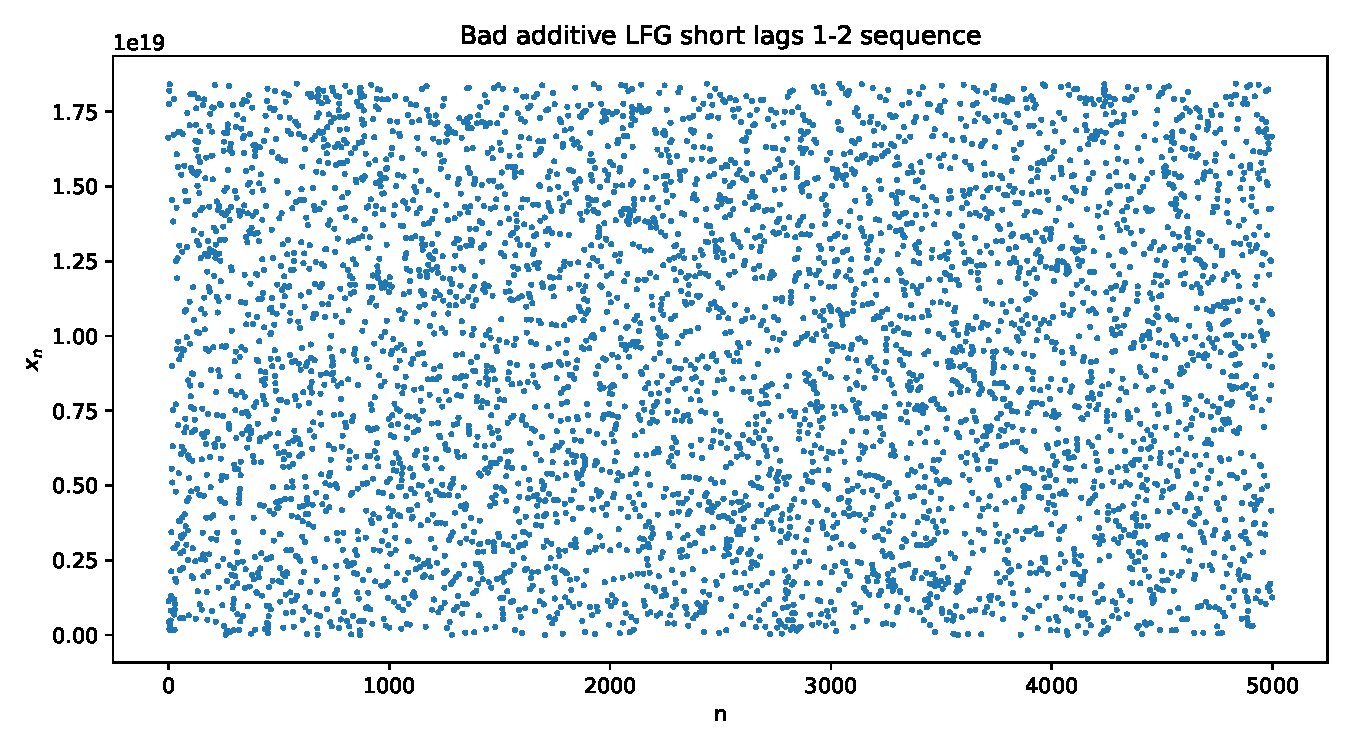
\includegraphics[width=0.48\textwidth]{figures/lfg/bad_large_range/lfg_bad_short_lags_1_2_sequence.pdf}
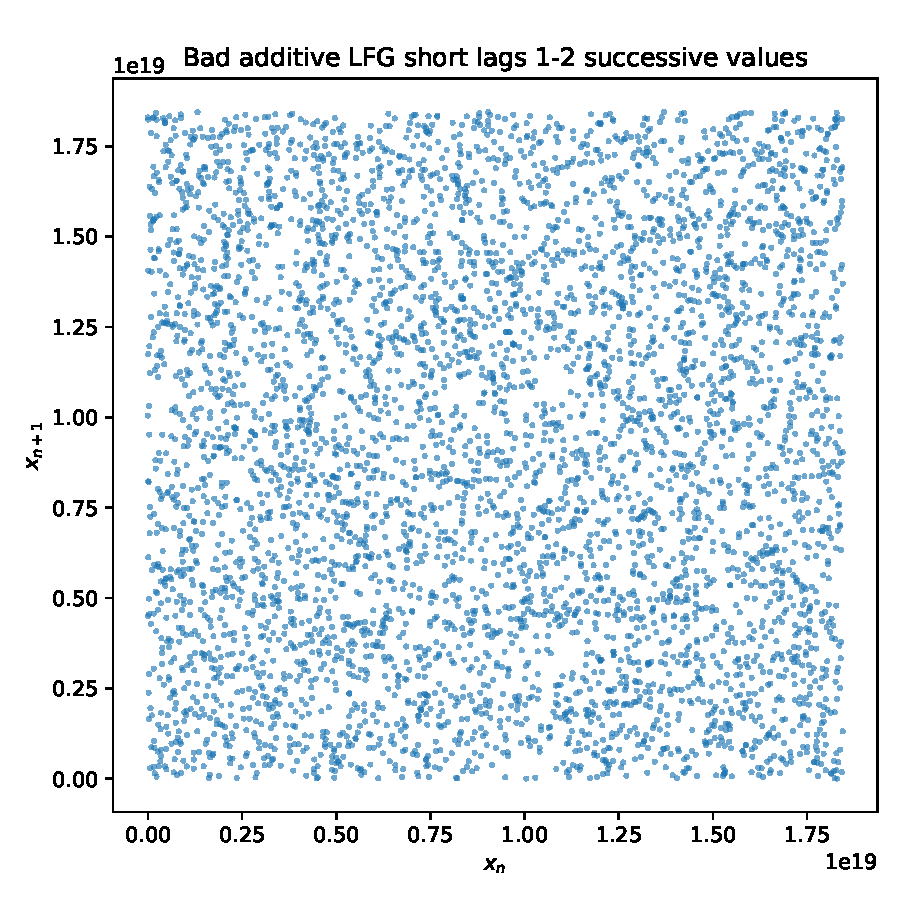
\includegraphics[width=0.48\textwidth]{figures/lfg/bad_large_range/lfg_bad_short_lags_1_2_successive_values.pdf}
\caption{Sequence plot and successive-value plot for the bad short-lag LFG}
\label{fig:lfg-bad-seq-succ}
\end{figure}

Figure \ref{fig:lfg-bad-seq-succ} shows stronger dependence between consecutive values than in the good case. Since the lags are too small, the generator behaves more like a simple Fibonacci recurrence than a well-separated lagged generator.

\begin{figure}[htbp]
\centering
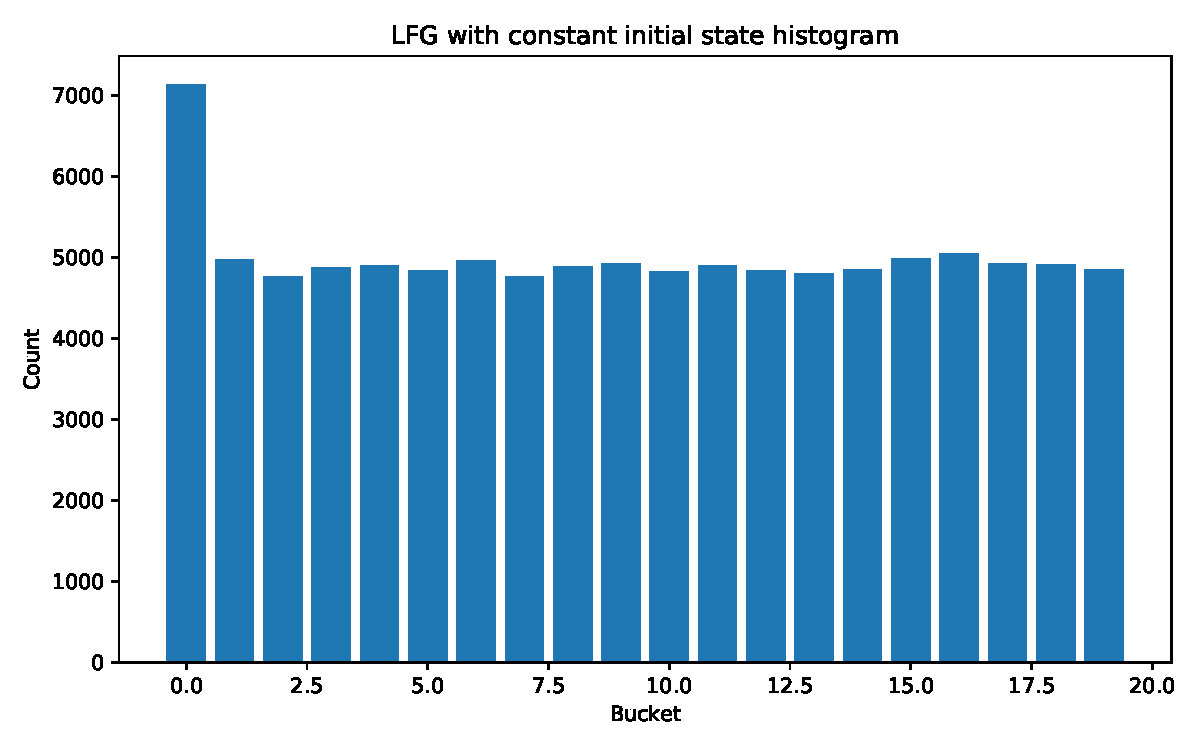
\includegraphics[width=0.48\textwidth]{figures/lfg/single_bad_parameter/lfg_single_bad_constant_state_histogram.pdf}
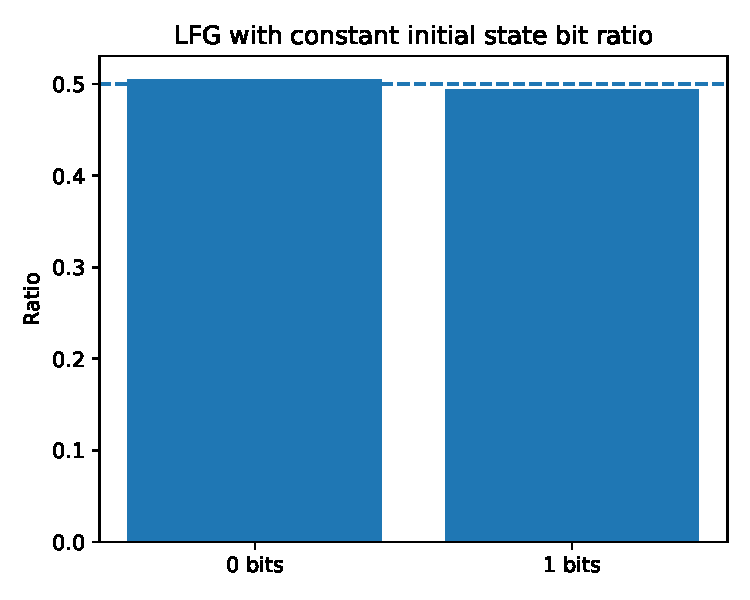
\includegraphics[width=0.48\textwidth]{figures/lfg/single_bad_parameter/lfg_single_bad_constant_state_bit_ratio.pdf}
\caption{Histogram and bit ratio for the LFG with constant initial state}
\label{fig:lfg-single-bad-hist-bits}
\end{figure}

Figure \ref{fig:lfg-single-bad-hist-bits} shows that a bad initial state can strongly damage the distribution. The chi-square statistic is much larger than in the good case, and the bit ratio is visibly shifted away from $0.5$.

\begin{figure}[htbp]
\centering
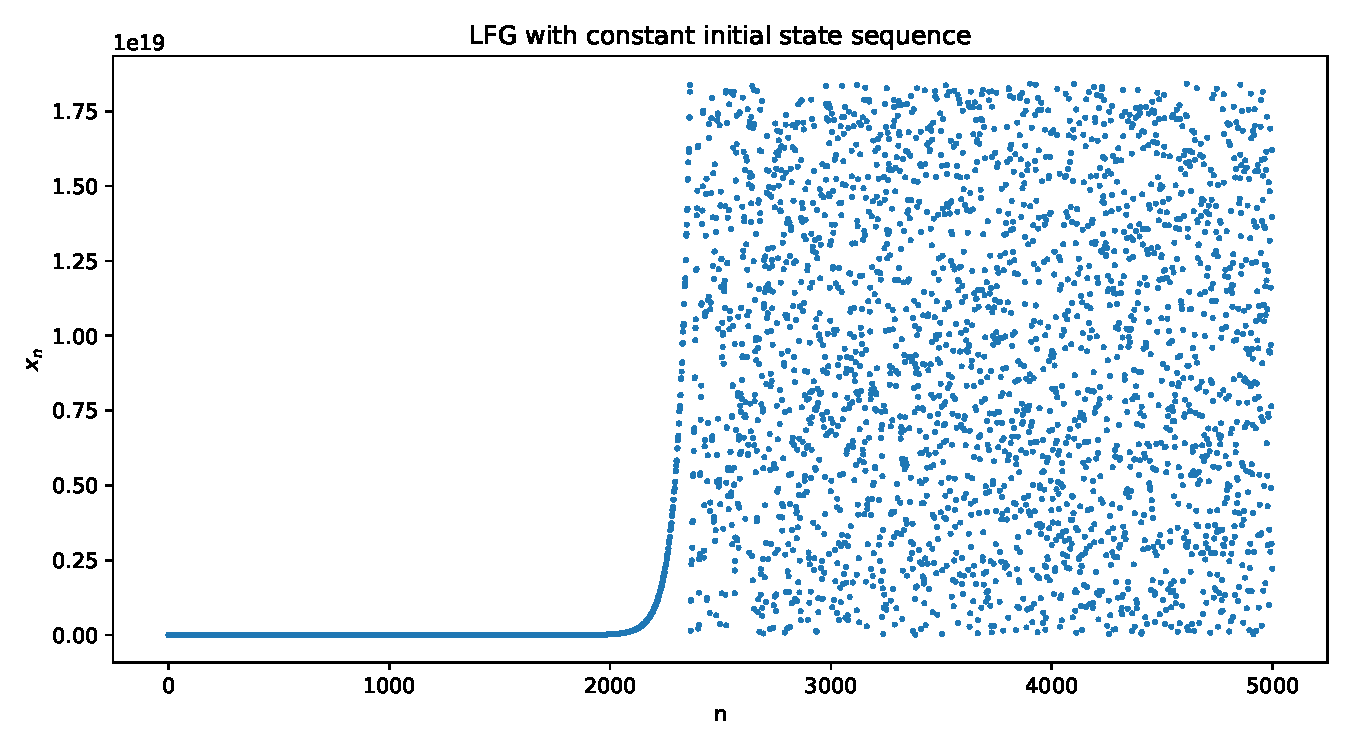
\includegraphics[width=0.48\textwidth]{figures/lfg/single_bad_parameter/lfg_single_bad_constant_state_sequence.pdf}
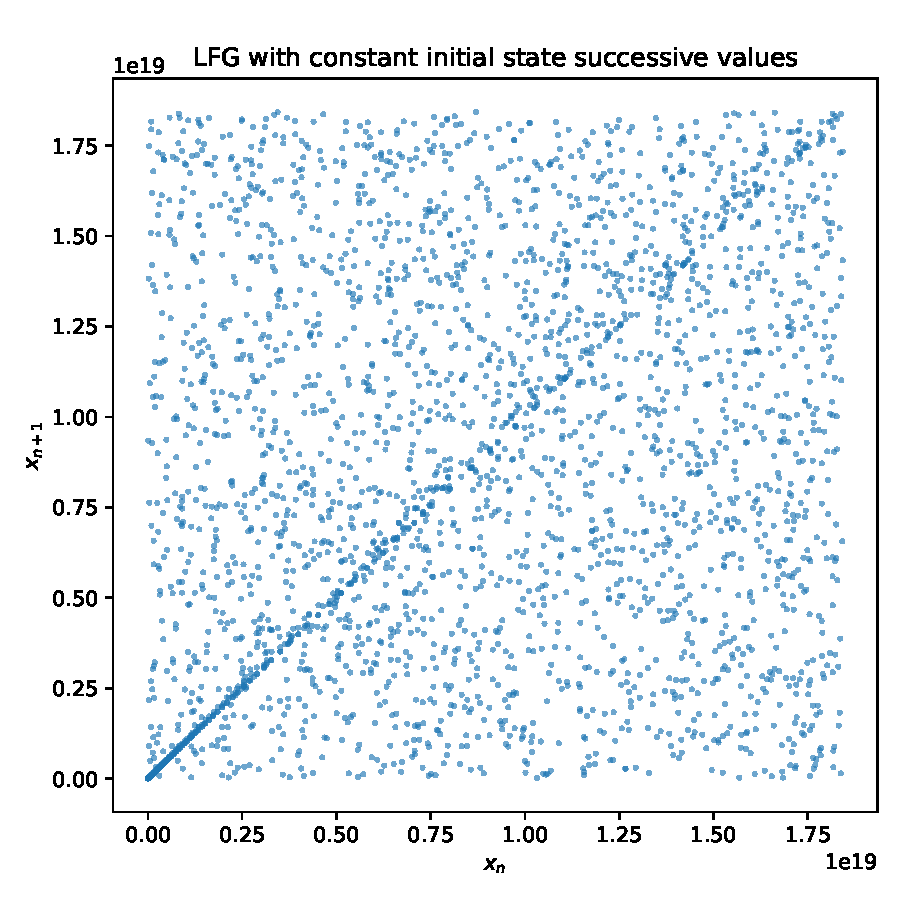
\includegraphics[width=0.48\textwidth]{figures/lfg/single_bad_parameter/lfg_single_bad_constant_state_successive_values.pdf}
\caption{Sequence plot and successive-value plot for the LFG with constant initial state}
\label{fig:lfg-single-bad-seq-succ}
\end{figure}

Figure \ref{fig:lfg-single-bad-seq-succ} confirms that initialization is part of the generator design. Even with reasonable lag values, starting from a poorly mixed state introduces visible structure. Therefore, LFGs should use both carefully selected lags and a non-degenerate initialization procedure.